\chapter{Background, Motivation, and Overview}\label{ch:background}

\section{Introduction to Prosody and Prosodic Annotation}\label{sec:introduction-to-prosody-and-prosodic-annotation}

%todo update bib so it’s 2022 instead of forthcoming for barnes+
In addition to being formed of words, spoken utterances contain a wide range of other information about timing, intonation, prominence, phrasing, voice quality, rhythm, etc., often collectively called spoken prosody. (See \citealt{ladd08}, \citealt{beckmanvenditti11}, and \citeauthor{barnesshattuckhufnagel20} \textit{forthcoming} for some broad overviews.) These aspects of an utterance are sometimes called supra-segmental, because they can span regions larger than a single phonemic segment (i.e., a single consonant or vowel). (See \citealt{lehiste70} for extensive discussion.)

In a language like English, two major categories of prosodic structure concern \textbf{prominence} (related to notions of accent, stress, focus, emphasis, etc.) and \textbf{phrasing} (related to notions of grouping, disjuncture, pauses, etc.). In turn, both prominence and phrasing correlate with changes in \textbf{pitch} (related to notions of f0, tone, intonation, etc.). Speakers of English modulate these and other prosodic aspects of speech and thereby signal distinctive pragmatic, semantic, syntactic, or morphological information. In order to study these phenomena, linguists and speech scientists of many types are interested in annotating the prosodic structure of utterances.

As an example of the effect of prosodic manipulation on linguistic structures and meanings that speech scientists and linguists have been interested in, consider the English string “\langtext{Steve or Sam and Bob will come}”. As discussed in \citealt{lehiste73} (also \citealt{price-91}, \citealt{veilleux-06}), manipulating the supra-segmentals that signal prominence and grouping in this sentence can change its fundamental meaning. In the following two pronunciations, capitalization indicates prominence and commas indicate phrasing.

\begin{enumerate} \def\labelenumi{\arabic{enumi}.}
\item STEVE, or Sam and BOB, will come.
\item Steve or SAM, and BOB, will come. \end{enumerate}

This simple manipulation of prominence and phrasing highlights the linguistic importance of prosody. Each of these two realizations of the same string (which are two of many possibilities) yields a fundamentally different structure and interpretation: the former is unclear about whether one or two people will come (Steve alone, or Sam and Bob together), while the latter more clearly communicates that two people will come and one of them will be Bob. Understanding this kind of prosodic patterning can be useful in a wide variety of domains, e.g., in formulating the linguistic grammar, modelling human speech production and perception, mapping prominence and grouping patterns to meaning differences, understanding the effects of prominence and grouping on the pronunciation of words, developing better-performing algorithms for automatic speech synthesis, recognition and translation, and improving understanding of speech disorders that involve prosody. To address these goals, researchers in intonation (and prosody more generally) need to be able to systematically annotate a variety of prosodic differences, in ways that go beyond laboratory examples and stylized productions, and capture aspects of the phonetic implementation of phonological prosodic contrasts.

\subsection{Pitch Cues to Prominence and Phrasing}\label{sec:pitch-cues-to-prominence-and-phrasing}

Though prominence and phrasing are abstract concepts, manipulation of the intonational acoustics of an utterance can provide strong cues as to which elements are prominent and where phrase boundaries exist.\footnote{The concept of prominence has been defined in a variety of ways, as required by different disciplines. For further discussion see \citealt{gussenhoven15}, \citealt{wagner-15}.} A particularly strong set of cues comes from changes in perceived pitch that are caused by changes in the frequency of vibration of the vocal folds (this vibration rate is often called “f0”, for “fundamental frequency”).\footnote{Note that the cues to phrasing and prominence are \textit{by no means} restricted to the acoustics of f0.  Speakers also manipulate dimensions such as duration, amplitude and voice quality (phonation quality) to signal prosodic structure. For some further discussion, see section \ref{sec:labelling-individual-cues}.} In terms of the meaning of a sentence, intonational differences can play a key role (as exemplified by sentences 1 and 2 above).

However, the relationship between pitch and meaning can be complex. For example, high pitch (acoustically measured as f0) can signal that a particular word is meaningfully prominent in English; however, ‘high pitch’ can map onto a wide range of f0 values in the acoustics, depending on context. This is because what counts as ‘high’ in one context, might be much higher\slash lower (in terms of f0 values) than what counts as ‘high’ in another. Moreover, it’s not just high f0 values that signal that a word is prominent in English; prominence can also be signaled by an f0 pattern that is low, rising, falling, or etc. In other words, there is no fixed 1-to-1 relationship between an f0 value and prominence.

In addition to signalling prominence, a high f0 can also be used to mark a phrase boundary, as in the pitch rise often heard on the final syllable of certain kinds of questions in English, such as “\langtext{Is it raining yet?}” Here, when f0 rises to a high value at the end of \langtext{yet} it does not necessarily mark a pitch-accented word; in fact, in perhaps most pronunciations of this question, \langtext{yet} is \uline{not} a phrasally-prominent word. Instead, a high f0 on \langtext{yet} can signal the presence of a phrase boundary following it.

The paragraphs above reveal that high f0 values can serve as cues to both prominence and phrase boundaries. Moreover, it is not always straightforward to determine whether a high f0 region serves as a cue to prominence or phrasing (or neither). Identifying these different \textbf{types} of f0 patterns (prominence- vs. phrasing-related) requires a theory (an intonational phonology), training, and often extensive practice. At the same time, one could --without knowing whether f0 changes are prominence- or phrasing-related-- annotate where significant changes in f0 trajectory (realized as, e.g., peaks or valleys) occur. PoLaR is designed with this goal in mind: It allows labellers to annotate perceptually-significant f0 changes separately from prosodic events like phrase boundaries and prominence, while still permitting annotation of these relationships where they are perceived to exist.

To summarize, prosody encompasses many different aspects of the speech signal -- beyond words and their phonological representations as sequences of consonants and vowels. Here we have focused on the intonational aspects of prosody, noting that PoLaR allows novice and advanced labellers to contribute differently to its annotation, according to their level of knowledge and their goals. This feature distinguishes PoLaR from some other prosodic annotation systems, which may have more fixed requirements based on a particular phonological theory of prosody.

\subsection{Terminology: f0, pitch, intonation, and prosody}\label{sec:terminology}

Before continuing, we will clarify our working definitions for some terms that are used throughout this monograph. We start with \textbf{f0} and \textbf{pitch}, because these two ideas are often conflated, especially in more casual discussion, even though there is an important difference between them. Fundamental frequency (f0) in speech is directly related to the rate of vocal fold vibration, and is estimated by signal detection algorithms in software like Praat. That is, what Praat calls the “pitch track” (shown in blue in the figures throughout this monograph) is more precisely an (estimated) f0 contour. On the other hand, pitch is not directly measurable - it is a psycho-perceptual phenomenon. As such, pitch only exists in the mind of a listener. To describe this another way, if there were a speaking event such that no one heard the speech, the utterance would have an f0 contour but no pitch, because pitch does not exist outside of the minds of a listener.

Both f0 and pitch are dynamic, changing in patterned ways over the course of an utterance. These dynamic changes are often visualized as a graph, where the x-axis represents time and the y-axis represents f0 values; the visualizations of f0 changes are correspondingly called \textbf{f0 contours} (a.k.a. “f0 tracks”). On the other hand, a more abstract representation of how a listener perceives pitch changes over time (e.g., a visualization like a straight line approximation) is called a \textbf{pitch contour}. Thus, an f0 contour is a description of changes in the \emph{f0 values} over time, while a \emph{pitch} contour is a description of changes in the perceived pitch over time. (Note that since, in our view, pitch does not exist without a listener with a mind to represent it, a pitch contour also does not exist without a listener with a mind.) Abstracting further over these contours, using discrete grammatical objects, produces what we call the \textbf{intonational contour}, which is an abstract sequence of pitch events (targets) that can occur over time in a spoken utterance.

This brings us to the term \textbf{intonation}, which we take to refer to the portion of phonetics\slash phonology that deals in describing\slash modelling patterns in pitch in linguistic utterances. To do so, intonation must make reference to various other aspects of phonetics and phonology, including other aspects of \textbf{prosody}. We take prosody to refer to the portion of phonetics\slash phonology that deals in describing\slash modelling patterns in suprasegmentals (i.e., patterns in the signal that can extend across multiple segments; see \citealt{lehiste70} for more discussion) in linguistic utterances. In other words, these definitions treat intonation as a subset of prosody. (At this point, it is worth mentioning that there are blurred lines in any conceptual distinctions here. The distinctions are blurry in part because the concepts are not discrete, because they interact with one another, and because colloquial usages of the terms are not always consistent.)

A summary of these working definitions is provided in the table below.

\begin{longtable}{>{\bfseries}p{.175\linewidth}p{.75\linewidth}} \endhead\toprule 
f0 &
a physical measure directly related to rate of vibration of the vocal folds, as reflected in the acoustic signal or articulatory measures
\tabularnewline\hdashline
pitch &
an abstract psycho-perceptual phenomenon related to f0 (\textit{requires a listener with a mind})
\tabularnewline\hdashline
f0 contour &
a description of changes in the f0 values in an utterance over time
\tabularnewline\hdashline
pitch contour &
a description of changes in pitch over time (\textit{represents events in a listener’s mind})
\tabularnewline\hdashline
intonational contour &
an abstract sequence of pitch events over time (\textit{requires a grammar})
\tabularnewline\hdashline
intonation &
the arm of phonetics\slash phonology dealing with pitch patterns
\tabularnewline\hdashline
prosody &
the arm of phonetics\slash phonology dealing more broadly with suprasegmental patterns
\tabularnewline\bottomrule 
\caption{Our working definitions for some commonly used terminology.
\label{tab:terminology}
}
\end{longtable}


\section{Motivation for PoLaR}
Those who are new to intonation and prosody should \textit{\textbf{feel free to skip this section}}. It is mostly aimed at positioning PoLaR in the literature on prosody and prosodic annotation. It has been written for an audience that is at least somewhat familiar with the issues of intonation (and prosody and suprasegmentals, more generally) as well as issues of already-established systems of annotating intonation.

\subsection{PoLaR Influences: Some Approaches to Prosodic Labelling}\label{sec:past-approaches-to-prosodic-labelling}

Systems for labelling prosodic information can vary from one to another, even in ways as fundamental as which aspects of the signal are attended to or the number of different symbols in the annotation ‘alphabet’. This holds even for annotation within a single language like English, and even for a single idealized variety of English, such as mainstream US English. In developing the PoLaR system, we have made extensive use of some of the concepts and ideas that have also been components of other labelling traditions:

\begin{itemize}
\item American structuralism (e.g., \citealt{pike45}, \citealt{tragersmith51}),
\item the British school (e.g., \citealt{crystal69}, \citealt{oconnorarnold73}),
\item the Dutch IPO model (e.g., \citealt{t-hart-90}), and
\item the Autosegmental-Metrical framework (e.g., \citealt{pierrehumbert80}, \citealt{beckmanayers97}, \citealt{grabe-01}, \citealt{hualdeprieto16}, \citealt{dilleybreen18}),
\item among others (e.g., \citealt{hirst07}, \citealt{taylor98}, \citealt{xu12}).
\end{itemize}
%todo add something about dima?

(For further description of past prosodic models and annotation systems, please see, e.g., \citealt{roach94}, \citealt{ladd08} Chapters 1 and 2, \citealt{fery17} Chapter 5, \citeauthor{barnesshattuckhufnagel20} \textit{forthcoming}.) That said, \uline{\textbf{no} familiarity with these systems is required in order to learn and apply the basic aspects of PoLaR annotation}.

\subsection{Context and Motivating Questions}\label{sec:context-and-motivating-questions}

PoLaR was developed in the context of many discussions over long periods of time, in which labellers well-versed in intonational annotation grappled with how to decide on the appropriate intonational label for certain contours (particularly in English), and in particular cases where the crucial differences appeared to involve considerations that are not always explicitly acknowledged. 
%
%todo revisit the flow here
%NOTE 22/7/1: the remainder of this paragraph used to be a footnote. make sure it sounds good in the text.
{In particular, the present authors have been involved in the development, instruction, and maintenance of the MAE\_ToBI system (\textit{M}ainstream \textit{A}merican \uline{E}nglish \uline{To}nes and \uline{B}reak \uline{I}ndices; \citealt{beckmanhirschberg94}, \citealt{beckmanayers97}, \citealt{beckman-05} currently embodied in MIT’s Open Courseware system [\href{https://ocw.mit.edu/courses/electrical-engineering-and-computer-science/6-911-transcribing-prosodic-structure-of-spoken-utterances-with-tobi-january-iap-2006/}{link}]). While committed to the development of PoLaR, the authors remain interested and invested in ToBI annotation systems for labelling phonological categories; we believe the systems are complementary, and not in competition. ToBI is a phonological annotation system, for transcribing intonational categories. It was developed within the framework of AM (\uline{A}utosegmental-\uline{M}etrical) phonology (as in \citealt{pierrehumbert80}, \citealt{ladd08}, \citealt{arvanitifletcher20}), which distinguishes different levels of prosodic phrases (e.g., “Intermediate Phrases” and “Intonation Phrases”), as well as different types of pitch movements (those associated with stressed syllables [e.g., “Pitch Accents”] and those associated with prosodic phrase edges [e.g., “Phrase Accents and Boundary Tones”]). While PoLaR can distinguish such objects, it doesn’t require that its labellers commit to any particular phonological analyses. In this sense it contrasts with ToBI, in which all phonological categories of pitch are annotated as either categorically high (H) or low (L), following \citealt{pierrehumbert80}).}

These discussions reflected the sense that, while existing (AM-based) phonological models of English intonation (e.g., MAE\_ToBI) are well-suited to capture many phonological aspects of the intonation system, they purposefully avoid capturing the finer details of intonation contours (and other aspects of prosody).  Because these details may be systematically determined, and furthermore may possibly signal additional categories and meanings, it became clear that a way needed to be found to permit their annotation. In particular, three questions emerged from these extensive discussions that have ultimately shaped the PoLaR system:

\begin{center}
\renewcommand{\arraystretch}{1.5}
\begin{tabular}{>{\raggedright\arraybackslash}p{.85\linewidth}}
\textbf{Three Motivating Questions}\\
\hline
\textbf{Question 1}: Which phonetic cues does\slash should a labeller attend to in labelling phonological categories?\\
\textbf{Question 2}: What is the range of possible suprasegmental phonetic implementations for a given phonological category?\\
\textbf{Question 3}: What are the ways in which prosody signals meaning, inclusive of and perhaps even beyond the phonological categories of current systems?\\
\end{tabular}
\end{center}


\textbf{Question 1}) \textbf{Which cues?} Labellers using phonological systems must still attend to acoustic cues, in order to determine which phonological label to use. At the same time, different labellers may make use of different cues and weight them differently (or even disregard them completely), leading to different phonological labels for the same observed set of cues. One of the motivations for developing PoLaR was to facilitate discussions of how each labeller interprets cues, by having them explicitly annotate the cues they attend to -- in PoLaR’s case, the intonational cues.  (See \ref{sec:labelling-individual-cues} in Chapter \ref{ch:beyond} for further discussion.)

\textbf{Question 2}) \textbf{What range of surface forms?} There is still much to be learned about the range of surface forms that can be used to signal a particular phonological category of pitch accent or edge tone - even for well-studied languages like English. PoLaR adds explicit focus on the acoustic details of the signal, so that a corpus with both PoLaR labels and more complex phonological (e.g., ToBI, RaP, IViE) labels will provide an inventory of surface phonetic realizations of each proposed phonological category.

\textbf{Question 3}) \textbf{Which meanings?} Despite decades of study of how prosody contrastively conveys meaning, it is not entirely certain that any existing phonological system of prosodic annotation captures all of the phonological categories of the prosodic system. For example, developments in the literature suggest that certain aspects of English intonational contours currently not captured by MAE\_ToBI labels may be particularly relevant for signaling semantic-pragmatic meanings (e.g., range size [cf. \citealt{ladd94}] and or certain boundary-related movements [cf. \citealt{ahn-16}]), beyond those signaled by the presence and type of pitch accents and hierarchical phrase boundaries. It is important to understand the ways in which meaning is affected, so as to better understand which acoustic changes are categorical, in a phonological sense.

%TODO integrate these reviewer comments
% THESE COMMENTS COME FROM P.6 OF THE REVIEWER COMMENTS
%That way, PoLaR nicely contributes to recent debates on how intonational categories may be best captured and defined (e.g., Arvaniti, 2019; Grice, Ritter, Niemann, & Roettger, 2017; Lohfink, Katsika, & Arvaniti, 2019; Roessig, 2021; Zahner-Ritter et al., 2022).
%This question is indeed not trivial, since the intonational realization of utterances is generally characterized by variation. Providing a tool to annotate phonetic information which may vary in a meaningful way and be linguistically relevant is hence of utmost importance.
%For instance, in a study by Grice et al. (2017), speakers of German consistently employed f0 alignment and scaling (in a phonetic sense) to differentiate between different focus types, so did speakers in Braun (2006) to mark contrastively used topics.
%Another case in point is a recent study by Zahner-Ritter et al. (2022) which tested whether and how three different rising-falling contours in German map on existing phonological events (L+H* vs. L*+H). The study provides evidence from form and function that speakers of German consistently distinguish an “intermediate contour” that acoustically lies between L+H* and L*+H. 
%I would thus support the authors’ claim that PoLaR can be used to explore category-internal variation to “uncover new phonemic distinction” (p. 128). In its attempt to capture the phonetic variation in the signal to determine its linguistic relevance PoLaR is hence a timely approach.
%Other systems, such as DIMA (Deutsche Intonation: Modellierung und Annotation, Kügler, Baumann, & Röhr, 2022; Kügler et al., 2015), account for similar questions. Compared to the German ToBI system and other systems of annotation (Grice et al., 2005; Kohler, 1991; Mayer, 1995; Niebuhr, 2022), DIMA is also more faithful to the signal, providing a way to analyse prominences and tonal events separately from each other; the authors may want to draw comparisons between the systems to underline their merits for the community. They also might want to comment on how applicable the system is to other languages.


To address these motivating questions, PoLaR provides tools for the annotation of an utterance’s acoustic qualities (targeting its prosodic phonetics) as well as some fundamental abstract aspects of its prosodic categories (targeting its prosodic phonology). PoLaR has been designed so that the task of labelling is not burdensome to the labeller (in a way that is especially useful to the novice). One way that this has been achieved is by designing the labels so that acoustic cues and abstract categories can be labelled separately from one another. Another way that this has been achieved is that the categories invoked are rather abstract (e.g., “prominent”) are kept to a minimal number, allowing a degree of neutrality with respect to specifics of the prosodic phonology of the language. At the same time, PoLaR is also useful for those with experience in intonational analysis and theory: the PoLaR Advanced labels permit the annotation of which phonetic details are (in the judgment of the labeller) related to the phonological categories of phrase-level prominences (pitch accents) and boundaries (edge tones).

The guidelines chapters of this monograph focus on the annotation of intonational phonetic details in particular (via the Points, Levels, and Ranges tiers), and so note that whenever we say “phonetics” or “acoustics” here, we primarily are referring to intonational phonetics and acoustics.  However, the annotation framework we use with PoLaR gives us the ability to expand annotation methods to similarly capture other domains of phonetic cues (timing, amplitude, phonation, etc.) that are relevant to prosodic structure. (We return to how to extend PoLaR in Chapter \ref{ch:beyond}.)

\section{The PoLaR system}\label{sec:polar-system}

\subsection{PoLaR Tiers and A Labelled Example}\label{sec:polar-tiers-and-a-labelled-example}

Some primary goals of PoLaR are:

\begin{enumerate}
\item to annotate a wider array of prosodically relevant features of speech than is possible in existing systems;
\item to isolate different prosodically relevant aspects of the speech signal from one another; and
\item to make the labelling task easier, by requiring fewer phonological decisions.
\end{enumerate}

An example annotated according to the PoLaR labelling guidelines is given in Figure \ref{fig:PoLaR 1st basic}.

\begin{figure}[H]
\centering
%
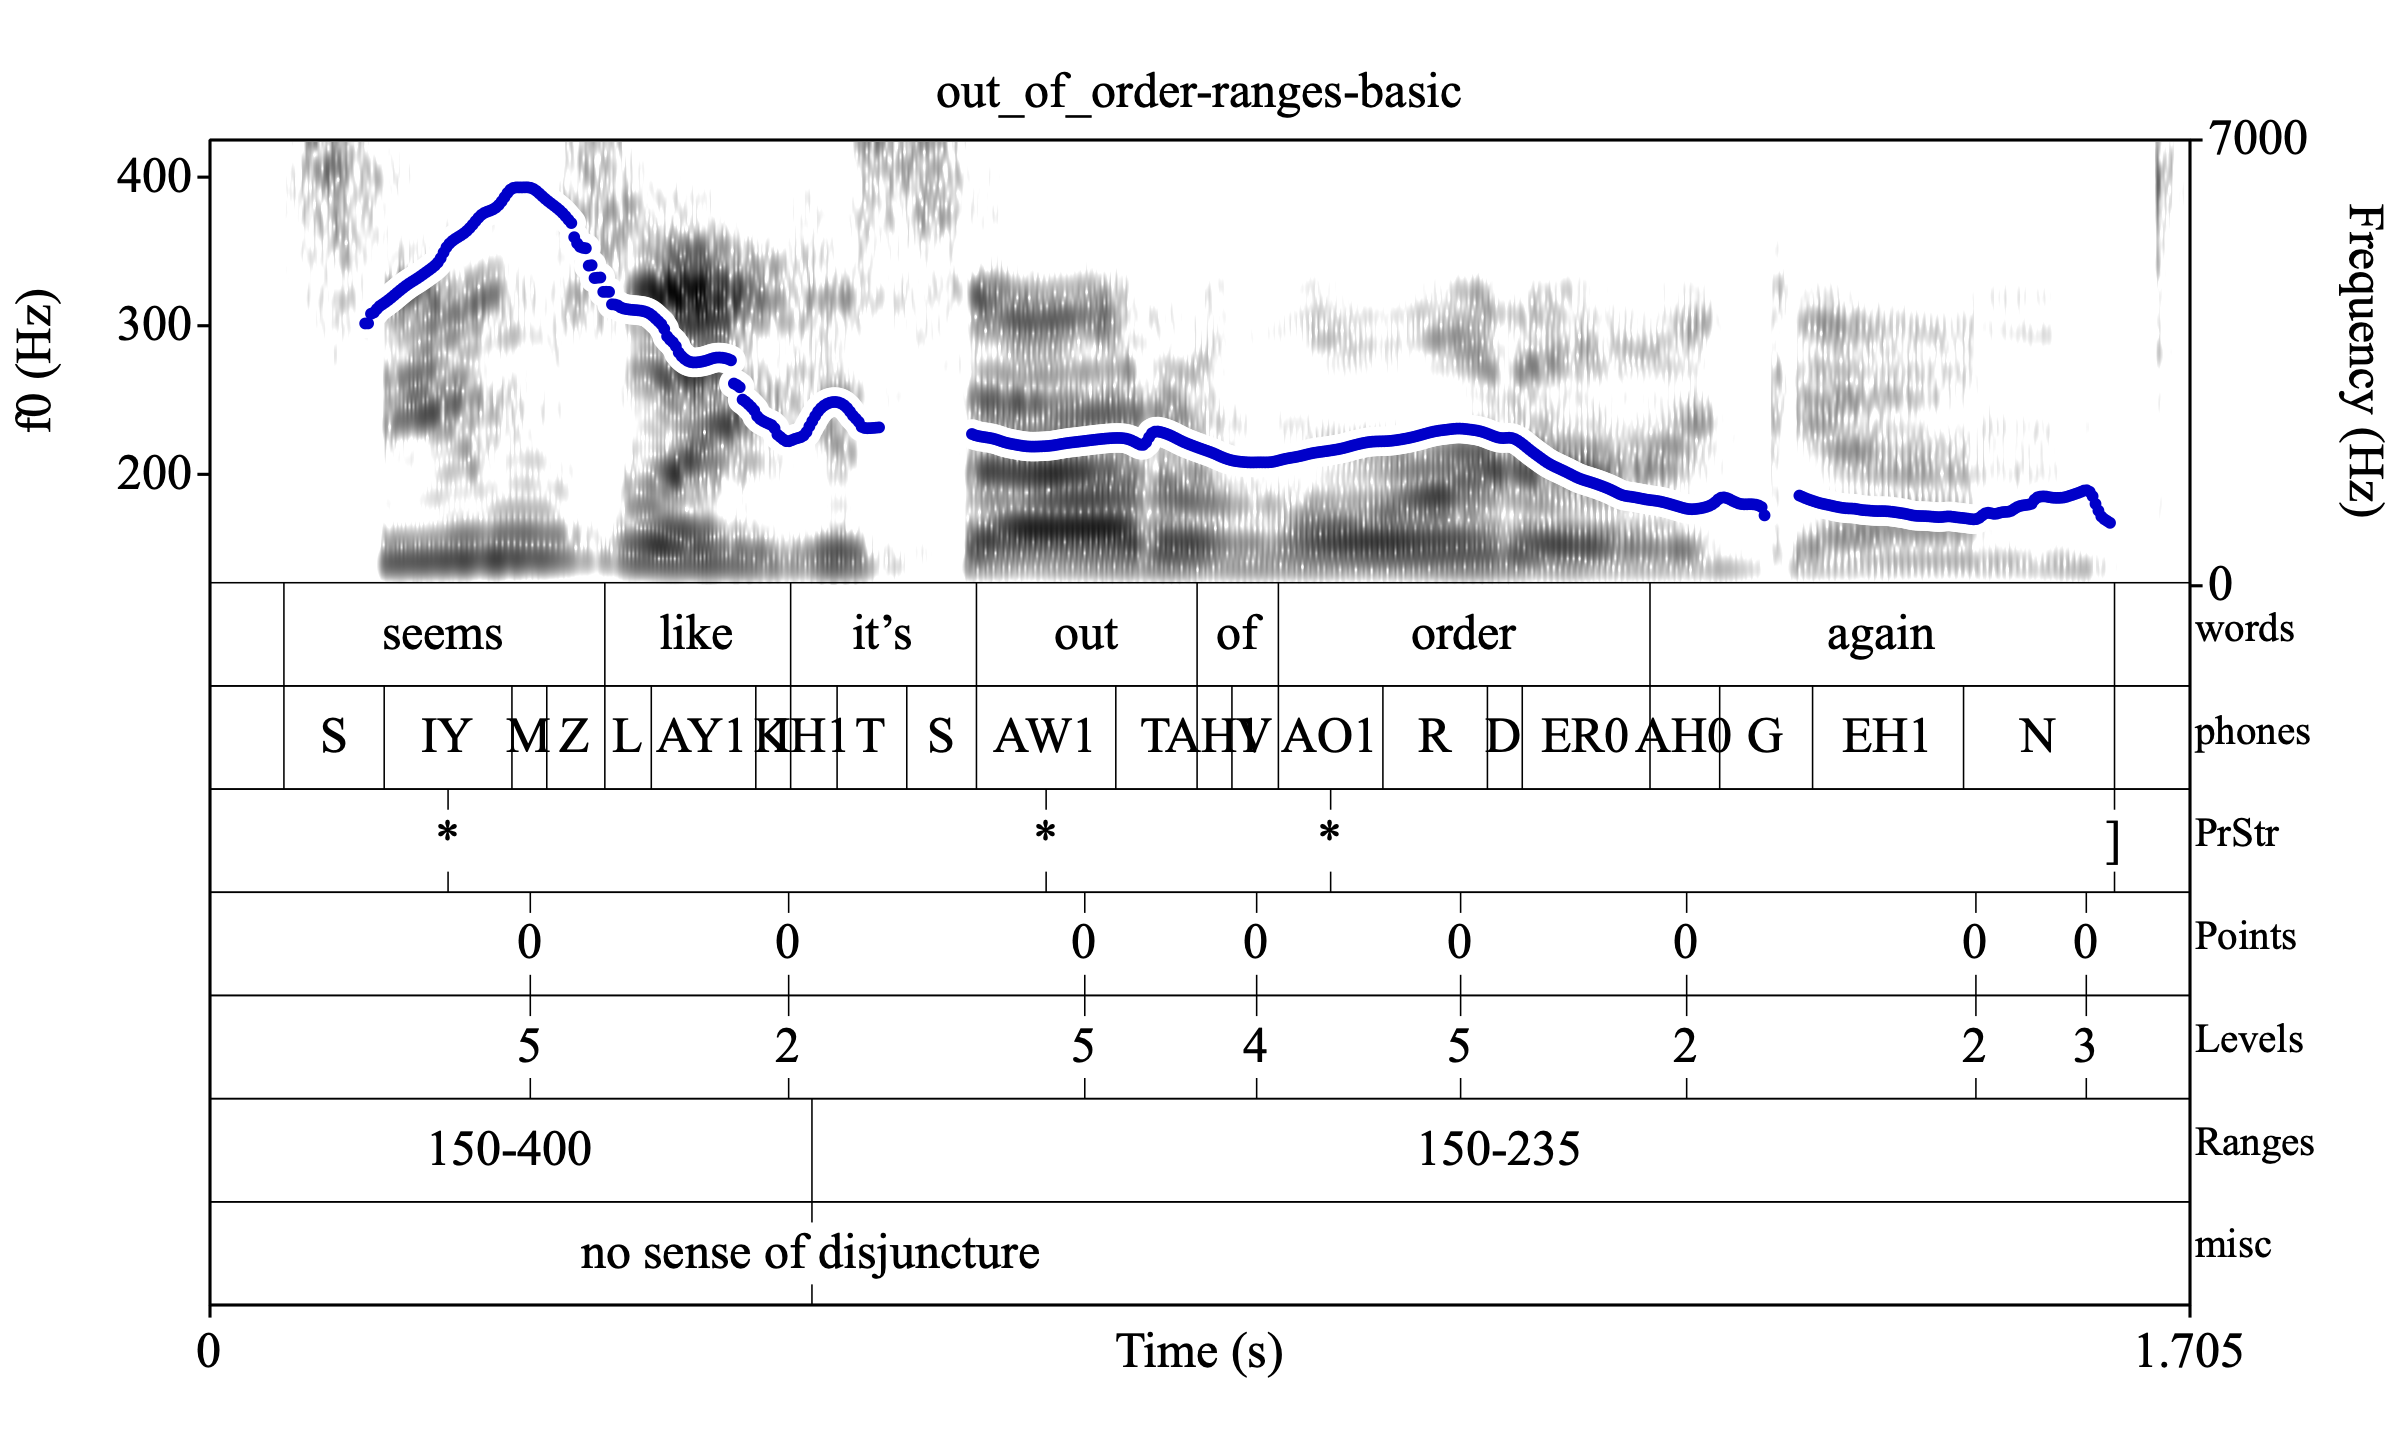
\includegraphics[width=.875\linewidth]{out_of_order-ranges-basic--7.png}
%
\caption{A recording annotated with Basic PoLaR labels. Note that the Phones tier is created automatically by the Montreal Forced Aligner (\citealt{mcauliffe-19}).\protect\footnotemark%
\label{fig:PoLaR 1st basic}%
\index{Annotated example, PrStr tier (basic)!out\_of\_order-ranges}
}
\end{figure}\footnotetext{The inclusion of a Phones tier does not reflect the authors’ commitment to the idea that phones have representational reality as bounded linguistic constituents.}


There are four core tiers of prosodic annotation (the third through sixth tiers in Figure \ref{fig:PoLaR 1st basic} above), described in these guidelines: three acoustic tiers (Pitch \textbf{Po}ints, Scaled \textbf{L}evels, \textbf{a}nd \textbf{R}ange Domains), and one phonological tier (Prosodic Structure).

\begin{enumerate} \def\labelenumi{\arabic{enumi}.}
\item The \uline{Prosodic Structure (PrStr) tier} is a point tier, and each label indicates the presence of a perceived prosodic prominence or a perceived prosodic phrase boundary. Prominence labels are placed in the middle of the vocalic nucleus of a prominent syllable, and boundary labels at the end of the last word of a prosodic phrase.
\item The \uline{Pitch \textbf{Po}ints tier} is a point tier, and each label corresponds to a turning point that the labeller observes in the f0. “Turning point” refers to any point in the f0 curve that looks to be a place where the f0 curve’s slope changes significantly (i.e., peaks, valleys, and the edges of plateaus).\footnote{PoLaR emphasizes the labelling of f0 turning points, because they are important aspects of an f0 contour, but this does not imply a commitment to an equivalence between turning points and intonational targets. See section \ref{sec:TCoG} on Tonal Center of Gravity for further discussion.} PoLaR also permits labellers to \textit{optionally} annotate, for each f0 turning point, which (type of) phonological object from the Prosodic Structure tier it is associated with. This tier is the aspect of PoLaR that requires the most substantial discussion, in part to establish which slope changes are significant, what types of ‘decoy’ or apparent f0 turning points can be ignored, and how missing turning points can be inferred; see section \ref{sec:points} for this discussion.
\item The \uline{Scaled \textbf{L}evels tier} is a point tier, and has a 1-to-1 relationship with the Points tier, in terms of the number and time alignment of annotations. That is, for each point in the Points tier, a point is added to the Levels tier, and that Levels tier object is labelled with a numerical value that corresponds to where in the current pitch-range (see 4 below) the turning point is. This tier is \textbf{automatically derived} from the Pitch Points Tier and the Range Domains tier, using the Levels labeller function of the PoLaR plugin for Praat.
\item The \uline{\textbf{R}ange Domains tier} is an interval tier, which captures a local pitch range for each utterance or section of an utterance. This annotation makes it possible to define the “high” and “low” for a particular stretch of an utterance, which is more explicitly manifested in the labels of the Scaled Levels tier (as in 3 above). For Basic PoLaR labels, the max\slash min for each Range interval is used to determine the numerical Levels values automatically inserted in the Levels tier. \end{enumerate}

Some PoLaR labels are phonological in nature (though also somewhat underspecified; e.g., “prominence” or “phrase boundary”), while others are more phonetic (e.g., f0 turning points). Annotating each tier only requires attention to one stream of suprasegmental properties (e.g., the Points tier only identifies f0 turning points); this allows each tier to be annotated on its own.\footnote{Note that no tier requires bundling information from multiple prosodic domains into a single label (this contrasts with a label like \textlabel{H*}, which bundles together prominence, pitch height, f0 turning points, etc.). Some Advanced labels re-connect these separated-out features; this is discussed at length for the Points tier in Chapter \ref{ch:advanced}.\label{fn:no bundling}}

PoLaR thus \textit{\uline{explicitly}} annotates both categories (phonology) and acoustic cues (phonetics), but with these streams of information \textit{\uline{separated from one another}}. We believe that annotating this information separately will reduce confounds in analysis and uncertainty in labellers. As we will see when discussing each tier in more detail, Advanced labels can be used to relate information on the phonological tier to information on the multiple phonetic tiers.

\subsection{Why These Tiers?}\label{sec:why-these-tiers}

The design choice of all labels and tiers (even these more phonetic ones) is, to some degree, phonologically informed and language-specific. That is, PoLaR labels do not identify just “any old (phonetic) information”, but rather information that is likely to be relevant for models of English intonation: e.g., pitch alignment, pitch height, prominence, and pitch range. These tiers and labels were chosen by the designers of PoLaR, based on experience with English intonation, but researchers who want to use PoLaR in another language may need to recalibrate the specific labels and/or tiers that get implemented. Because PoLaR is a framework for exploring the categories and cues to intonational prosody, rather than a fixed set of elements to be labelled, the number and nature of the tiers is extendable to accommodate the needs of particular studies. The following paragraphs review the thinking behind the design choices for each tier.

\uline{PrStr:}\\ Following AM theory (cf. \citealt{pierrehumbert80}), we assume that there are different types of intonational events, which are associated with different types of abstract phonological objects. In particular, we assume the now classic view that there are two basic sorts of phonological objects in prosodic structure that have direct influence of intonational contours: those related to intonational prominence and those related to intonational phrasing. (To be clear, the term ‘intonational prominence’ is meant to invoke a level of ‘post-lexical’ prominence: prominence higher than the level of lexical stress; cf. \citealt{bolinger58}, \citealt{libermanprince77}, and \citealt{beckmanedwards94}.) By design, all of the labels on this tier avoid indicating anything about how they are acoustically realized tonally - even abstractly. For example, differences like \textlabel{H-} vs. \textlabel{L-}, or \textlabel{H*} vs. \textlabel{L*} are purposely not captured at all in these labels. (These f0 properties will be captured by other labels on other tiers.) While these phonological objects can be signalled by a variety of cues (including changes in f0, duration, intensity, voice quality, etc.), none of these cues are themselves described by labels on this tier. Instead, what is transcribed is only the labeller’s \textit{\textbf{perception}} of prominence and phrasing. In this way, these Prosodic Structure tier labels are intentionally agnostic about the range of potential acoustic realizations of these different phonological objects. This method encodes information similar to that encoded by \citeauthor{cole-14}’s \citeyear{cole-14} Rapid Prosody Transcription method (RPT), and was influenced by their proposal. In RPT tasks, listeners mark perceived boundaries and prominences without concern for precisely how they are realized. This means that data gathered with an RPT methodology could be automatically translated into the accent and boundary tone markers on the Prosodic Structure tier. Labelling PrStr is designed to be simpler than other prosodic labelling systems, with the goal of allowing others to more easily understand the original labeller’s intentions.

\uline{Points:}\\ The f0 turning points in an f0 contour play an important role in many different theories.  For example, researchers have attributed a relationship between f0 turning points and phonological elements, either directly (e.g., as peaks, valleys, or anchored elbows; see, e.g., \citealt{ladd-99} and \citealt{welby06}) or indirectly (e.g., as important factors in implementing f0 shape and alignment distinctions, as in the Tonal Center of Gravity work of \citealt{barnes-12} et seqq.). For these reasons, it is useful to determine where they are.  Unfortunately, at the moment this cannot be done automatically, but requires human intervention, for several reasons.  First, f0 is challenging to track automatically, and there are often “missing” turning points (e.g. during voiceless segments or creaky-voiced regions).  Second, it is challenging to determine which turning points are significant, and which should in contrast be regarded as ‘decoy’ points: either too small to make a perceptible difference, or the result of a tracking error.  Thus, human labelling of points defined as significant for perception of intonation is required, and this monograph provides guidance for determining significant turning points, identifying decoys and inferring missing points.  See section \ref{sec:optional-f0-override-labels-for-annotating-pitch-points-without-a-reliable-f0-track} in Chapter \ref{ch:basics} for further discussion.

While it is widely agreed that there is a mapping relationship between the types of objects in our Prosodic Structure tier and the f0 turning points of the Points tier, PoLaR does not commit its labellers to any particular analysis of this relationship. In this way, the labeller need not try to keep the phonological model in mind while labelling the Points tier, nor even be familiar with any phonological model. At the same time, PoLaR provides a way for labellers to annotate the relationship between the two tiers. (How to do this is laid out in Section \ref{sec:optional-advanced-labels-for-relating-points-tier-objects-to-prosodic-structure-tier-objects} in Chapter \ref{ch:advanced}.) In this way, the Points tier can also be used for annotating mappings between acoustic events and phonological objects.

\uline{Levels:}\\ The Levels tier allows PoLaR to capture the relative height of a Points tier object (on a scale of 1 to 5). This relative height can be useful for analysis, since a raw f0 value does not by itself indicate whether that value is high or low (in the speaker’s current intended range). This is because, as noted earlier, a relatively low f0 in the speaker’s full possible f0 range may be functionally\slash phonologically high if the speaker’s current f0 range is low, and vice versa. The Levels tier encodes scaled pitch values for each f0 turning point on the Points tier. That value corresponds to the pitch quintile in which it occurs (1 being the lowest quintile and 5 being the highest), with the boundaries for each pitch quintile being calculated on the basis of the pitch range annotated in the Ranges tier. Annotators should use the PoLaR plugin for Praat to automatically have Levels annotation added, once Points and Ranges tiers have been annotated. Further discussion can be found in chapter \ref{ch:practical}.

\uline{Ranges:}\\ The Ranges tier reflects that f0 events are always interpreted within a speaker’s range--not only their overall speaking range, but within locally determined ranges. The Ranges tier provides the context in which the levels (i.e., on the Levels tier) reflect individual points on the Points tier. That is, this is used to identify whether an f0 point is “high”, “low”, or somewhere in between, in the context of a particular utterance or part of an utterance. The Ranges labels require human labellers because we need intuitions on which parts of the pitch are perceived to be H or L in the speaker’s range. The Ranges tier can be used to capture and reflect the relations and differences among pitch events, both locally within a range, and across ranges.

Labelling Ranges tiers in this way allows analyses that other AM labelling systems do not: relative heights between pitch ceilings\slash floors in arbitrarily distant parts of the recording can be compared. In AM labelling systems, the pitch range can only be inferred by looking at the labelling and the recording together, alongside a theoretical model of the relationship between phrasing and acoustic measures (e.g., that new intermediate phrases begin new pitch ranges). Such an inference can lead to problems in cases where the labeller and the reader have different assumptions about the relationship between phrases and pitch ranges. This highlights the PoLaR system’s core, laid out in the introduction: it keeps track of information that other intonational annotation systems make use of, but differently from those other systems, it requires that such information be tracked \emph{explicitly}.

\section{Overview of PoLaR’s Advantages}\label{sec:overview-of-PoLaRs-advantages}
Before delving into the details of the system, we describe here several general points about the advantages of PoLaR. Its primary goal is to identify the melody of a spoken utterance; in this sense it has something in common with the IPO approach (so named for the Dutch the Institute for Perception Research, ‘Instituut voor Perceptie Onderzoek’), which produces straight line approximations by connecting turning points (\citealt{t-hart-90}), which can serve as a proxy for key aspects of the melody.  In particular, PoLaR has been designed to have five useful characteristics: Compatibility, Flexibility, Modularity, Accessibility, Expandability, Crosslinguistic usability, and Explicitness; in addition, it has inspired concomitant development of a useful set of Associated Tools. 

\paragraph{Compatibility with other annotation systems / prosodic analyses:}
PoLaR works well with other labelling tools and systems which have different goals, and its use alongside other annotation systems is encouraged; PoLaR is not intended as a complete model of spoken prosody.  For example, parallel PoLaR and e.g. ToBI\footnote{ToBI annotation systems exist for a number of languages and varieties; see \citealt{jun05, jun14} for works describing ToBI systems for a number of languages.} labels can be expected to shed light on both the phonemic inventory of a language and the phonetics-phonology interface. 

For these reasons, PoLaR is not intended as a replacement for other annotation systems. As such, PoLaR can be seen as a supplement to existing systems (such as the ones mentioned in Section \ref{sec:past-approaches-to-prosodic-labelling}). At the same time, it can stand alone, and PoLaR labellers need not have any familiarity with other prosodic annotation systems.

\paragraph{Flexible for different research goals:}
The PoLaR system, which builds on existing frameworks and labelling systems, was developed to enable both (1) more detailed descriptions of languages with well-studied intonational phonology, in particular with reference to the capture of acoustic details of intonation for which the linguistic relevance has not yet been determined, and (2) the annotation of phonetic patterns in languages, dialects, or varieties whose phonology has not yet been explored, as a step toward understanding the intonational grammar. Its minimal invocation of language-specific phonology adopts prominence and boundary locations from AM theory, and it focuses on acoustic characteristics that are, according to human judgment, relevant for linguistic signalling (\citealt{barnesshattuckhufnagel20}).   

At its core, a PoLaR annotation is a phonologically-informed (but maximally theory-neutral) labelling of intonational acoustic-phonetic cues. This description brings to the forefront the fact that PoLaR labels are neither purely phonetic, nor purely phonological; instead, they are intended to capture phonologically relevant acoustic aspects of the speech signal. Thus, what is perhaps most important here is the separation between labels for phonological objects from phonetic labels of the acoustic characteristics that serve as cues to those objects, as well as the separation of different acoustic cues each to its own tier, and explicit labelling of more of these acoustic characteristics. We believe the labels that we provide below for each of the proposed labelling tiers are a good starting point for US English varieties, but exemplify what PoLaR annotation can do for any language or variety.

\paragraph{Modularity / “Unbundled” labels:}
In PoLaR, acoustic-phonetic cues and phonology are annotated separately. (And the phonological labelling is minimal, specifying (in its basic form) only the location of prominences and boundaries.) This reflects design principle: PoLaR \textbf{disentangles different types of information} as much as possible - isolating different components of prosody on different tiers of annotation. This unbundling facilitates decision-making during labelling, by requiring only minimal phonological awareness on the part of the labeller. (This stands in contrast with phonological labels that bundle together prominence, pitch alignment and scaling, etc.) This unbundling allows PoLaR to be annotated one at a time (at least with the Basic labels in Ch.\ref{ch:basics}), without the need to consider the labels on other tiers - this allows for a ‘divide and conquer’ approach to the labelling task, in which individuals can specialize in specific tasks, in an assembly line model.

At the same time, for those advanced labellers who are interested in connecting labels to a prosodic theory, PoLaR also provides ‘Advanced’ labels (Ch.\ref{ch:advanced}), to allow a labeller to annotate some relationships between tiers. This may facilitate exploration of how prosodic components on one tier relate to components on another. (See Extensibility below.)

\paragraph{Accessibility of use:}
PoLaR has been designed to be \textbf{easy to start using}, with relatively minimal instruction, so that useable data of particular interest to a researcher can be produced quickly.  This is in part because PoLaR does not require its labellers to have extensive knowledge of a phonological model of prosody, and in part because the different sets of labels are inherently module (allowing some labellers to be only trained in one area of prosodic labelling).

PoLaR’s modularity and lack of reliance on prosodic phonology stands in contrast to existing systems which do not specify how precisely to map labels onto particular sets of cues, and thus do not enable straightforward investigation of how different speakers (and labellers) use different cues in different contexts, or of what cues speakers use to signal particular contrastive intonational categories.

Because of this accessibility, the tasks of labelling different tiers can be split among different labellers, who can quickly develop expertise in that area.  In this way, the first steps of the labelling process are intermediate between the full training process for phonological labelling and the training-free method of Rapid Prosody Transcription (RPT) described in \citet{cole-14, cole-17}. 

Moreover, while accessible, the system requires that annotators using even the most basic PoLaR labels be explicit about their perception, intuition, and/or analysis - facilitating high-level discussions among more experienced or analysis-oriented users. (In addition, Advanced PoLaR labels allow such analysis-oriented users to systematically transcribe their analyses.)

\paragraph{Expandability of the annotation system:}
Although this monograph focuses on the \emph{intonational} aspects of spoken prosody, a critical feature of PoLaR’s design is that it does not restrict labellers to only annotating this information. To be clear, we mean that PoLaR annotation is broadly intended as a \emph{\textbf{framework}} (which is to say it is a way of conceptualizing annotation systems), so that there is not a rigid way for PoLaR annotation to be implemented. 

Instead, the particular implementation described in this monograph is intended to be seen as a narrow execution of broader conceptual ideas. A labeller can expand\slash contract the set of labels on a particular tier or expand\slash contract the set of tiers that are labelled, so as to adjust what aspects of prosody and cues to prosodic structure are annotated. For example, a labeller may wish to systematically annotate duration, intensity, or phonation cues. Or they may wish to annotate other aspects of prosodic structure, such as lexical stress, footing, etc. This is useful, because tabulating and understanding the individual cues to prosodic prominences and boundaries can provide important insights into how phonetic implementation of a phonological intonation category can vary (\citealt{brugos15, brugos-18}).

Labelling projects with different goals can also omit tiers that are judged to be less relevant, allowing a novice labeller to focus on (and become expert in) a particular aspect of the intonation.  In this way, more complex labelling tasks can be approached with a divide and conquer strategy, which allows each labeller to become expert and reliable more quickly. 

\paragraph{Crosslinguistic usability:}
PoLaR is designed to be usable for any language as well as for any speech style, register, or dialect \emph{within} a language. PoLaR’s focus on acoustic cues and broad phonological categories makes PoLaR useful in the initial stages of exploring a language or dialect whose prosody is under-\slash un-documented.  While some tiers require native speaker intuition (e.g., prominences, boundaries). others could be used without native speaker intuitions (e.g., turning points).  Thus, using PoLaR can be a step toward formulating a phonological transcription system of intonationally-undocumented systems.  This is critically important, because our current understanding of human speech prosody is based on analysis of a strikingly small proportion of the world’s languages, while at the same time, it has become easier to create corpora of recorded utterances in understudied languages for analysis.  Thus the time is right for development of a system such as PoLaR which facilitates getting a foothold on the analysis ladder for addressing a new language or dialect. 

Beyond work on understudied languages\slash dialects, PoLaR can also be useful for studying how suprasegmental cues are used differently across varieties and contexts, within a language\slash variety. Researchers working with a corpus that is annotated for demographic or contextual information could use PoLaR labels in much the same way as it would be used for crosslinguistic work.\footnote{For those wishing to create their own corpus, see, e.g., \citealt{meyerhoff-11} or \citealt{podesvasharma13} for some discussion of recording this sort of information as well as a description of some best practices.}

\paragraph{Explicitness of annotation:}
PoLaR facilitates discussion with respect to differences in labeller intuitions, through its explicit annotation of cues (such as f0 turning points and ranges). Discussions are also facilitated through the relationships described by Advanced labels, which can encode labeller intuitions about the connections across tiers (such as pointers in the Points tier to indicate the direction of affiliation to a phonological boundary or prominence). Similarly, it encourages the development and testing of hypotheses about systematic aspects of these relationships. For example, PoLaR facilitate analyses that reveal not only how each type of prominence and boundary proposed in a phonological theory of intonation can be realized acoustically in different contexts, but also whether the proposed contrastive categories would benefit from extension or revision.

\paragraph{Associated tools:}
A plugin has been developed that includes a set of scripts to facilitate the labelling process. (As described at several points throughout this monograph; it can be accessed through the OSF repository at \url{https://doi.org/10.17605/OSF.IO/USBX5}.) This plugin can do things such as helping a labeller determine whether a particular PoLaR label ought to be included, substantially facilitating the resolution of ambiguous cases. Other functions include automatically adding labels on particular tiers on the basis of other labels, and exporting information extracted based on the labels in a format that can be usable for statistical analysis and machine learning.  (For more discussion of this plugin, see Chapter \ref{sec:past-approaches-to-prosodic-labelling}.) Finally, the system benefits from integrating with existing tools, such as ones for phone segmentation by forced aligners (e.g. Montreal Forced Aligner, \citealt{mcauliffe-19}, downloadable from \href{https://github.com/MontrealCorpusTools/Montreal-Forced-Aligner}{MontrealCorpusTools on Github}; or the Penn Forced aligner, \citealt{yuanliberman08}, downloadable from the \href{https://web.sas.upenn.edu/phonetics-lab/facilities/}{Penn Phonetics Laboratory website}).

%todo add a section on places to be concerned?
% reviewer note:
%My second point is a methodological one regarding interrater reliability between labellers. The fact that the advanced version of PoLaR is very rich in its inventory and provides a wide range of possibilities for annotation (integration / linking of events etc.) makes it complex at the same time. My question is how well the system can be learned and how reliable annotations across annotators are (especially with regard to the Ranges Tier, see above). I think that a framework as comprehensive as PoLaR needs to provide the reader with information on such issues. It is a plus that PoLaR can be used by both novices and advanced labellers and that the book can be read selectively. Adding a chapter on interrater reliability studies (for both the basic and advanced approach) would substantially strengthen the manuscript and the annotation system as a whole.
	%> response: there are many places of labeller freedom that can yield problems, yes; ADVICE: researchers could document choices?



\section{Who Will Find PoLaR Useful}\label{sec:who-will-find-polar-useful}

This monograph describes a recently developed system for annotating prosody, PoLaR, which is  aimed at fulfilling some of the needs described above. PoLaR has been designed with some particular influences and goals in mind, as outlined in the next section. Before getting into the details of those goals, and how they differ from the goals of other annotation systems, we will suggest some circumstances in which we think PoLaR might be particularly useful.

\textbf{How much experience is required to become a user?} PoLaR has been designed to facilitate the labelling process, and to be useful for a wide range of individuals with different levels of experience, backgrounds, and goals. It is designed to require minimal theoretical knowledge, enabling \uline{novice labellers} to begin producing useful annotations more quickly. It is also designed for research groups where different individuals label different aspects of the signal, \uline{in parallel}. Lastly, advanced aspects of the system are designed to be useful for \uline{advanced labellers} or \uline{theoreticians}, who are interested in the finer details of the prosody.

\textbf{Which areas of research could benefit?} PoLaR was also designed to facilitate making new discoveries, especially with respect to how variation within prosody (and specific prosodic characteristics) relates to variation in a (linguistic and/or extra-linguistic) context. For this reason (alongside its usability for novice labellers), PoLaR will be useful for \uline{variationists}, \uline{sociolinguists}, \uline{acquisitionists}, \uline{semanticists\slash pragmaticists}, \uline{morphologists}, \uline{phonologists}, etc. --as well as those working at the interfaces-- to help understand how prosody relates to these domains. Because it facilitates the annotation of potentially systematic aspects of the acoustic detail of an intonational contour, it is well suited to exploratory analysis of both understudied languages and understudied varieties of familiar languages.


